% Defines the document class
\documentclass[10pt,portuguese]{beamer}

% Defines the theme
\usetheme{metropolis}

% Imports the pre-defined packages
\usepackage{styles/packages}

% Imports the pre-defined templates
\usepackage{styles/templates}

% Imports the pre-defined colors
\usepackage{styles/colors}

% Imports the first slide's header
\usepackage{styles/header}

% Defines meta-information about the presentation
\title{Augmentação de Dados Textuais}
\subtitle{Mini-Curso do ICMC/USP}
\date{\today}
\author{Gustavo de Rosa}
\institute{
    Universidade Estadual Paulista ``Júlio de Mesquita Filho" (UNESP)
    \\
    Faculdade de Ciências (FC) / Departamento de Computação (DCo)
    \\
    Bauru, SP - Brasil
}

% Finishes up the preamble definition and starts the document
\begin{document}

% Makes up the preamble slide
\maketitle

% Imports the corresponding slides
\begin{frame}{Sumário da Apresentação}
    \tableofcontents
    %\tableofcontents[hideallsubsections]
\end{frame}
\section{Introdução}
\label{s.introduction}

\begin{frame}{Introdução}
	Lorem ipsum ...
\end{frame}
\section{Processamento de Linguagem Natural}
\label{s.nlp}

\begin{frame}{Processamento de Linguagem Natural}
	\begin{itemize}
		\justifying	
		\item Quaisquer formas de comunicação, escrita ou verbal, carregam vastas quantias de informação, as quais podem ser utilizadas para \textbf{prever} o comportamento humano;
		\\~\\
		\item Tais informações \textbf{não} são \textbf{triviais} de serem analisadas, pois cada ser humano possui características inerentes à sua forma de comunicação.
	\end{itemize}
\end{frame}

\begin{frame}
	\begin{figure}[!ht]
		\centering
		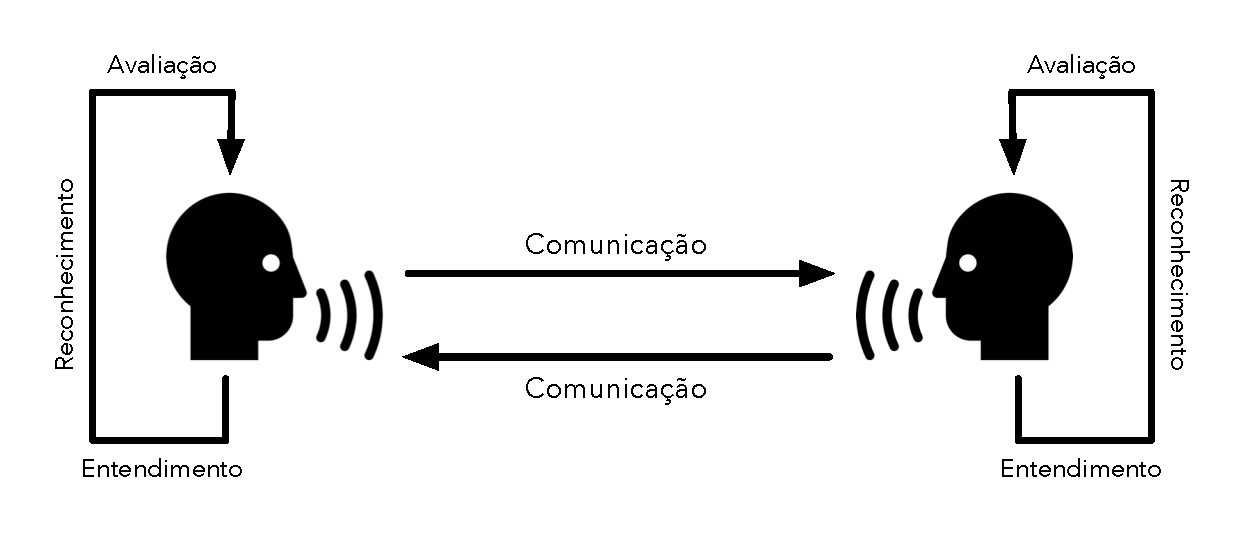
\includegraphics[scale=0.45]{figs/speech_workflow.eps}	
		\label{f.speech_workflow}
		\caption{Processo de comunicação simplificado entre dois seres humanos.}
	\end{figure}
\end{frame}

\begin{frame}
	\begin{itemize}
		\justifying
		\item O objetivo final de um sistema de Processamento de Linguagem Natural é \textbf{compreender e utilizar} uma linguagem da mesma forma que o próprio humano a utiliza;
		\\~\\
		\item Uma compreensão inteligível da linguagem humana requer um \textbf{discernimento} tanto de caracteres como de palavras e, ademais, como ambos estão conectados;
		\\~\\
		\item Enquanto humanos são capazes de aprender e masterizar uma linguagem facilmente, as máquinas ainda esbarram em suas características \textbf{ambíguas} e \textbf{imprecisas}.
	\end{itemize}
\end{frame}

\begin{frame}
	\begin{figure}[!ht]
		\centering
		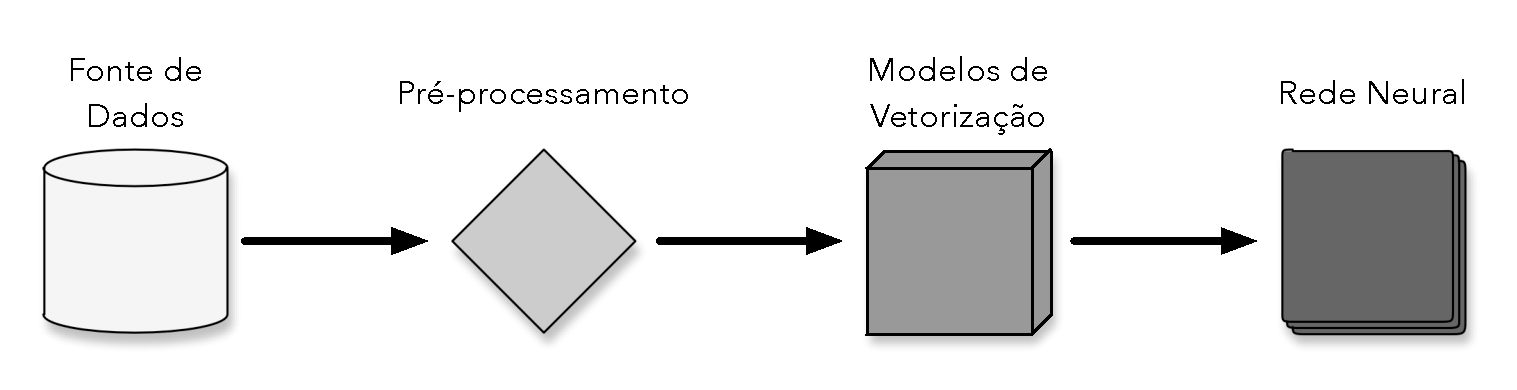
\includegraphics[scale=0.4]{figs/nlp_workflow.eps}	
		\label{f.nlp_workflow}
		\caption{Fluxograma da modelagem de um problema de Processamento de Linguagem Natural.}
	\end{figure}
\end{frame}

\subsection{Exemplos de Tarefas}
\label{ss.tasks}

\begin{frame}{Exemplos de Tarefas}
	\begin{itemize}
		\justifying
		\item Diálogo: Análise de discursos, resolução de correferências e sumarização automática;
		\\~\\
		\item \begin{sloppypar}Semântica: Análise de sentimentos, desambiguação de palavras, entendimento de linguagem natural, extração de relacionamentos, \textbf{geração de linguagem natural}, reconhecimento de entidades nomeadas, reconhecimento de vínculo textual, reconhecimento ótico de caracteres, semântica léxica, semântica distribucional, segmentação de tópicos, sistema de perguntas e respostas e tradução de máquina;	\end{sloppypar}
		\end{itemize}
\end{frame}

\begin{frame}
	\begin{itemize}
		\justifying
		\item Sintaxe: Análise gramatical, extração de terminologias, indução gramatical, lematização, marcação de partes da fala, quebra de sentenças, segmentação de palavras, segmentação morfológica e stemização;
		\\~\\
		\item Voz: conversor de texto para voz, reconhecimento de voz e segmentação de voz.
		\end{itemize}
\end{frame}

\begin{frame}
	\begin{figure}[!ht]
		\centering
		
\includegraphics[scale=0.4]{figs/nlp_applications.eps}	
		\label{f.nlp_applications}
		\caption{Exemplos de aplicações baseadas em Processamento de Linguagem Natural. Em sentido horário: \emph{Google Translate}, \emph{Microsoft Word}, \emph{Grammarly}, \emph{Cortana}, \emph{Siri}, \emph{OK Google}, \emph{Alexa} e \emph{IBM Watson}.}
	\end{figure}
\end{frame}

\subsection{Modelagem de Linguagem}
\label{ss.gln}

\begin{frame}{Modelagem de Linguagem}
	\begin{itemize}
		\justifying
		\item A tarefa de modelagem de linguagem refere-se à capacidade de modelos probabilísticos em \textbf{estimar} um $t+1$ estado dado $t$ estados anteriores;
		\\~\\
		\item O modelo linguístico aprende a \textbf{probabilidade de ocorrência} de \emph{tokens} baseado em exemplos;
	\end{itemize}
\end{frame}

\begin{frame}
	\begin{itemize}
		\justifying
		\item O processo de treinamento é baseado em um \textbf{conjunto de exemplos}, não sendo prático para estimar dados não-existentes, por exemplo, \emph{tokens} não encontrados no conjunto de dados;
		\\~\\
		\item Modelos linguísticos são utilizados como \textbf{arquiteturas-base} em tarefas complexas;
		\\~\\
		\item Também podem ser utilizados para a \textbf{geração artificial de texto}.
	\end{itemize}
\end{frame}

\begin{frame}{Geração Artificial de Texto}
	\begin{itemize}
		\justifying
		\item Um modelo linguístico \textbf{adequadamente treinado} é capaz de codificar características e regras do texto em que foi treinado;
		\\~\\
		\item Aprender a \textbf{distribuição probabilística} que representa o conjunto de dados utilizado.
	\end{itemize}
\end{frame}

\begin{frame}
	\begin{itemize}
		\justifying
		\item Distribuição probabilística de um \emph{token} no estado $t$, dado uma sequência prévia de $n$ \emph{tokens}:
		\begin{equation}
			P(w_t | w_{t-1}, w_{t-2}, \ldots, w_{t-n})	
		\end{equation}
		\\~\\
		\item Objetivo é estimar as probabilidades de um \emph{token} $w_{t+1}$ dado uma sequência prévia de $n+1$ \emph{tokens}:
		\begin{equation}
			P(w_{t+1} | w_{t}, w_{t-1}, \ldots, w_{t-n+1})	
		\end{equation}
	\end{itemize}
\end{frame}

\begin{frame}
	\begin{figure}[!ht]
		\centering
		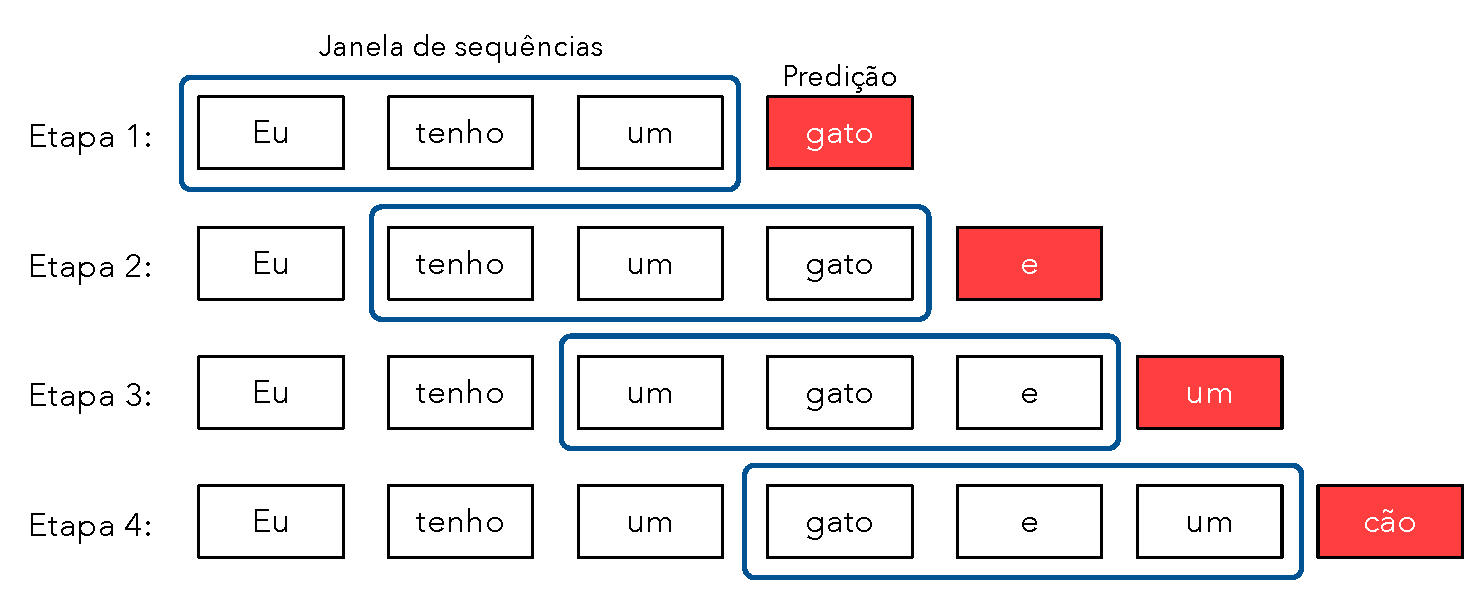
\includegraphics[scale=0.425]{figs/text_generation.eps}	
		\label{f.text_generation}
		\caption{Exemplo de um processo de geração artificial de texto.}
	\end{figure}
\end{frame}
\section{Redes Neurais Recorrentes}
\label{s.rnn}

\begin{frame}{Redes Neurais Recorrentes}
	\begin{itemize}
		\justifying
		\item Elman~\cite{Elman:90} propôs as Redes Neurais Recorrentes, do inglês \emph{Recurrent Neural Networks} (RNN);
		\\~\\
		\item Pertencem à uma categoria de redes em que a conexão entre seus nós forma um \textbf{grafo direcionado} ao longo de uma sequência;
	\end{itemize}
\end{frame}

\begin{frame}
	\begin{figure}[!ht]
		\centering
		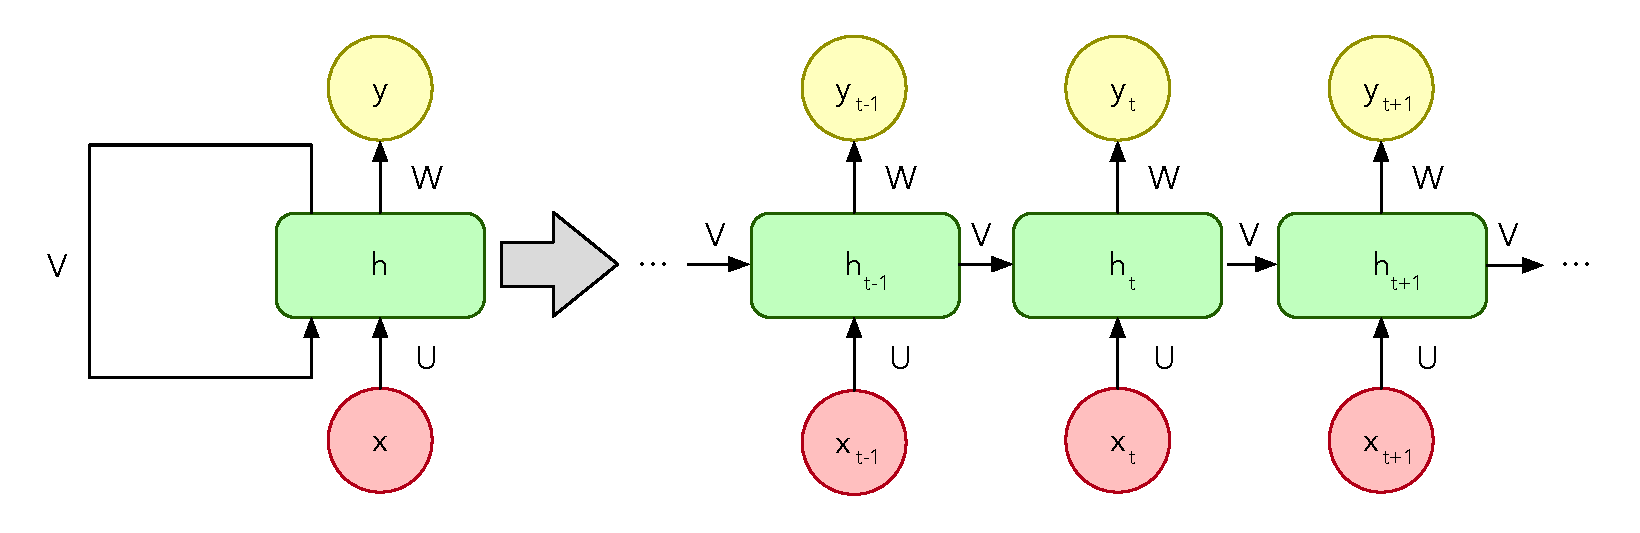
\includegraphics[scale=0.4]{figs/rnn.eps}	
		\label{f.rnn}
		\caption{Arquitetura básica de uma Rede Neural Recorrente.}
	\end{figure}
\end{frame}

\begin{frame}
	\begin{itemize}
		\justifying
		\item Utilização do fator tempo durante o treinamento pode acarretar no problema da \textbf{dissipação do gradiente};
		\\~\\
		\item Gradiente torna-se extremamente \textbf{pequeno} ao longo das iterações, prevenindo as atualizações de pesos;
		\\~\\
		\item Alternativa está na arquitetura em profundidade da \textbf{Rede de Memória de Longo Prazo}.
	\end{itemize}
\end{frame}

\subsection{Rede de Memória de Longo Prazo}
\label{ss.lstm}

\begin{frame}{Rede de Memória de Longo Prazo}
	\begin{itemize}
		\justifying
		\item Hochreiter et al.~\cite{Hochreiter:97} propuseram as Redes de Memória de Longo Prazo, do inglês \emph{Long Short-Term Memory} (LSTM);
		\\~\\
		\item Tipo especial de RNNs, explicitamente projetadas para aprenderem informações por \textbf{longos períodos} de tempo.
	\end{itemize}
\end{frame}

\begin{frame}
	\begin{figure}[!ht]
		\centering
		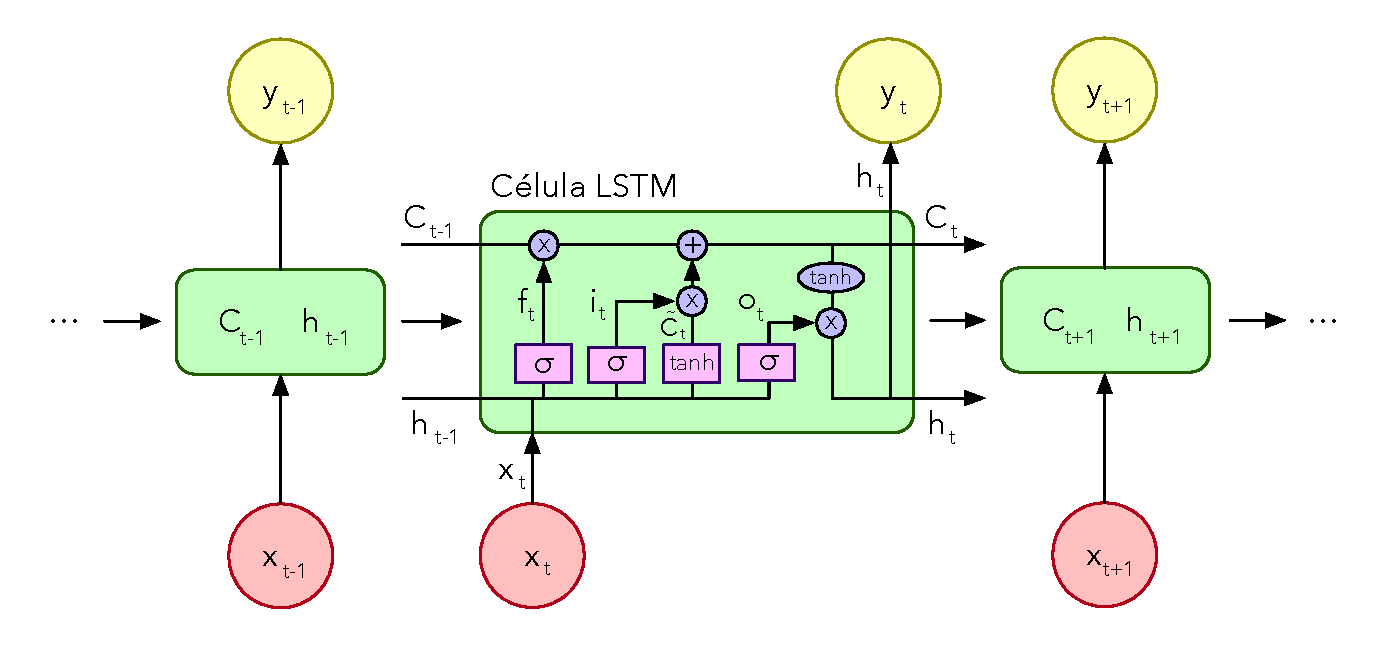
\includegraphics[scale=0.4]{figs/lstm.eps}	
		\label{f.lstm}
		\caption{Arquitetura de uma célula de uma Rede de Memória de Longo Prazo.}
	\end{figure}
\end{frame}

\subsection{Unidade Recorrente de Porta}
\label{ss.gru}

\begin{frame}{Unidade Recorrente de Porta}
	\begin{itemize}
		\justifying
		\item Cho et al.~\cite{Cho:14} introduziram as Unidades Recorrentes de Porta, do inglês \emph{Gated Recurrent Units} (GRU);
		\\~\\
		\item Também procuram solucionar o problema da dissipação ou estouro do gradiente e são vistas como variações das LSTMs.	
	\end{itemize}
\end{frame}

\begin{frame}
	\begin{figure}[!ht]
		\centering
		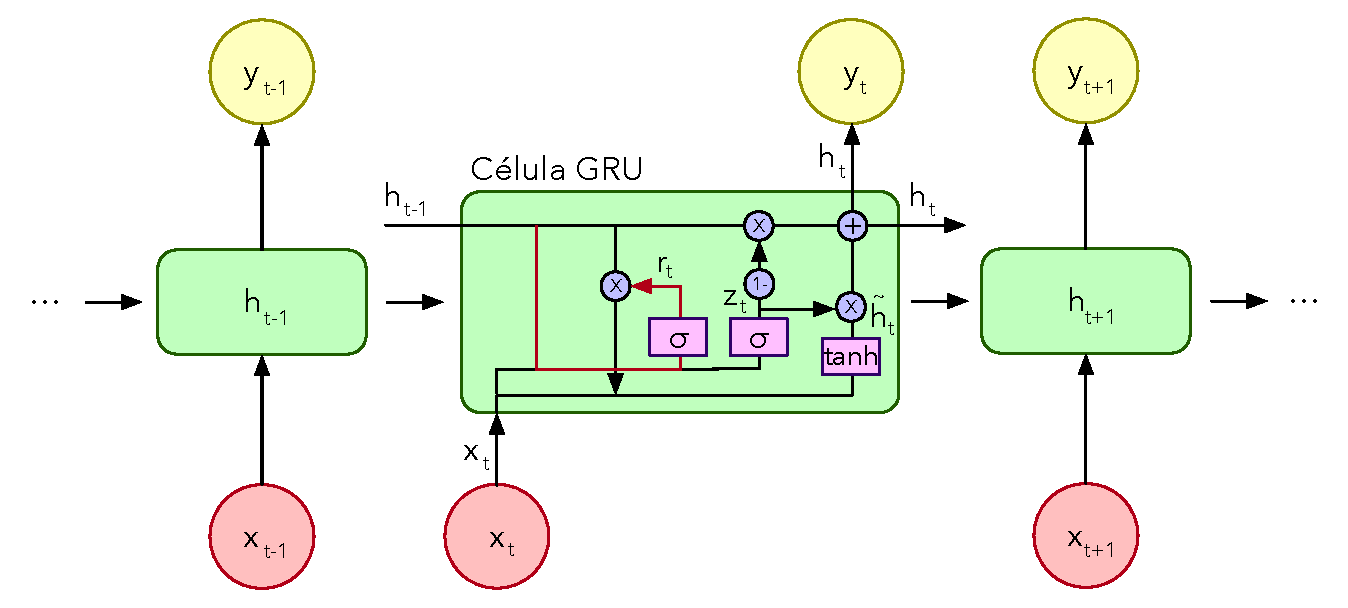
\includegraphics[scale=0.4]{figs/gru.eps}	
		\label{f.gru}
		\caption{Arquitetura de uma Unidade Recorrente de Porta.}
	\end{figure}
\end{frame}
\section{Transformadores}
\label{s.transformer}

\begin{frame}{Transformadores}
	\begin{itemize}
		\justifying
		\item Vaswani et al.~\cite{Vaswani:17} propuseram a primeira arquitetura de Transformadores, do inglês \emph{Transformers};
		\\~\\
		\item São arquiteturas puramente baseadas em mecanismos de Atenção e alternativas às Redes Neurais Recorrentes;	
	\end{itemize}
\end{frame}

\begin{frame}
	\vspace*{0.5cm}
	\begin{figure}[!ht]
		\centering
		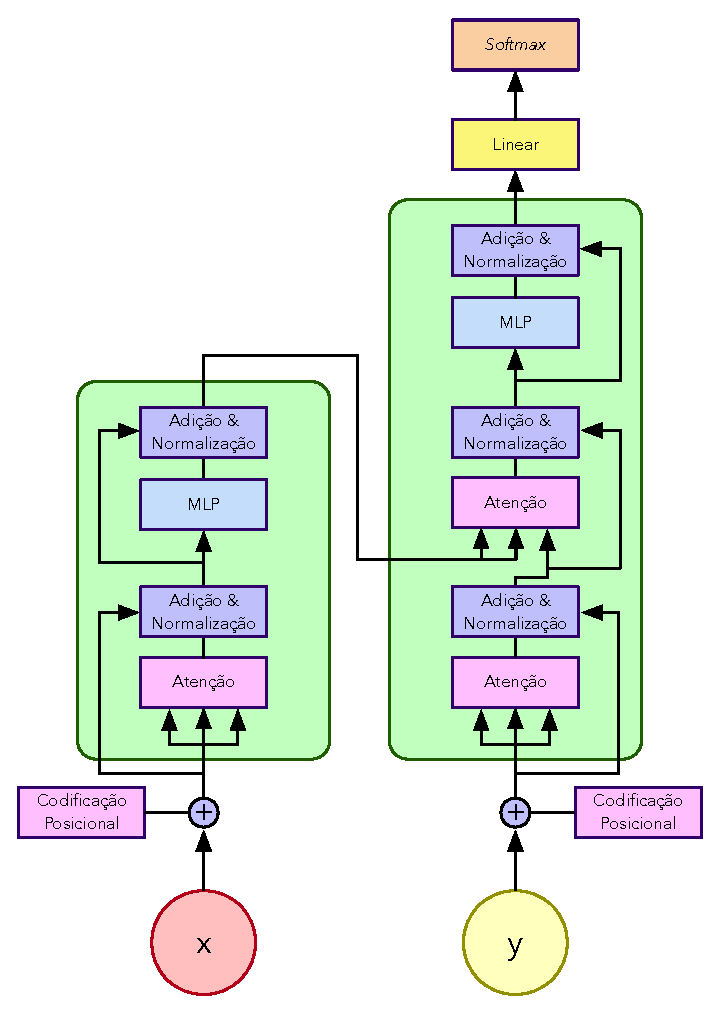
\includegraphics[scale=0.45]{figs/transformer.eps}	
		\label{f.transformer}
		\caption{Arquitetura de um Transformador.}
	\end{figure}
\end{frame}

\begin{frame}
	\begin{figure}[!ht]
		\centering
		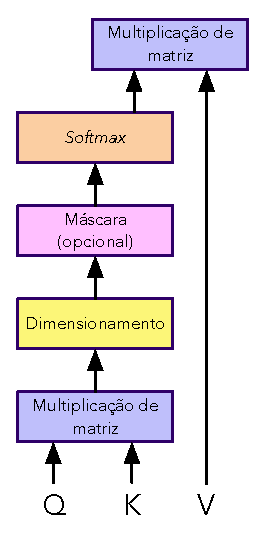
\includegraphics[scale=0.65]{figs/attention.eps}	
		\label{f.attention}
		\caption{Mecanismo de Atenção.}
	\end{figure}
\end{frame}


\begin{frame}
	\begin{figure}[!ht]
		\centering
		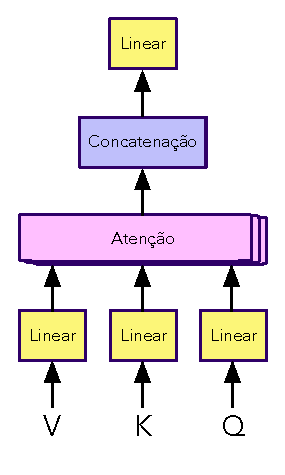
\includegraphics[scale=0.75]{figs/multi_head_attention.eps}	
		\label{f.multi_head_attention}
		\caption{Atenção de Múltiplas Cabeças.}
	\end{figure}
\end{frame}

\section{Aplicações}
\label{s.application}

\begin{frame}{Aplicações}
	\begin{itemize}
		\justifying
		\item Modelagem de Linguagem com Máscaras;
		\\~\\
		\item Modelagem de Linguagem Causal;	
		\\~\\
		\item \emph{Bot} para Augmentação de Dados.
	\end{itemize}
\end{frame}

\begin{frame}{Modelagem de Linguagem com Máscaras}
	\begin{figure}[!ht]
		\centering
		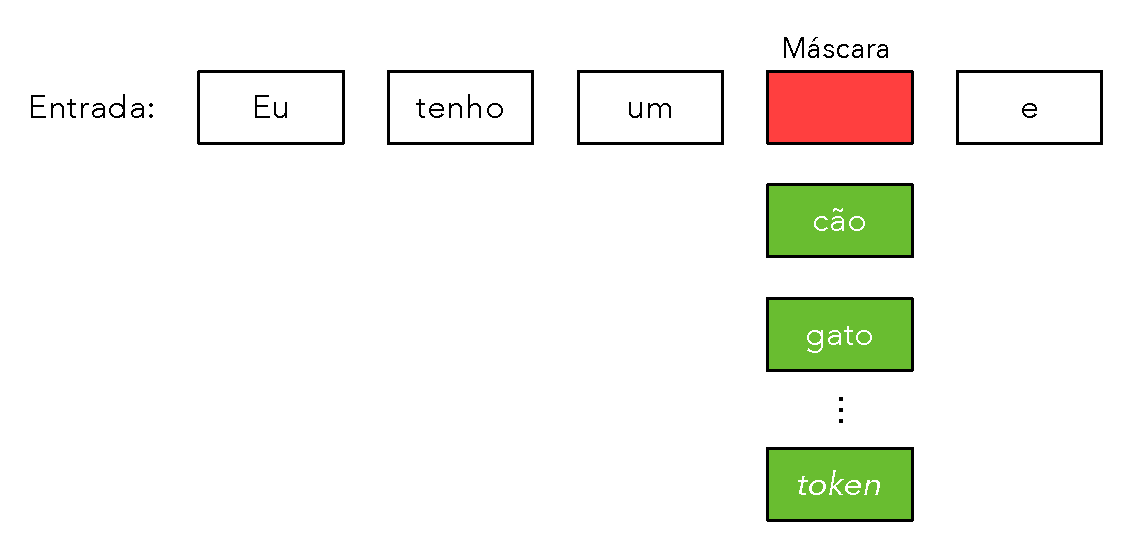
\includegraphics[scale=0.45]{figs/masked_lm.eps}	
		\label{f.masked_lm}
		\caption{Processo de modelagem de linguagem com máscaras.}
	\end{figure}
	Código: \url{https://github.com/gugarosa/text_augmenter/tree/master/applications/masked}
\end{frame}

\begin{frame}{Modelagem de Linguagem Causal}	
	\begin{figure}[!ht]
		\centering
		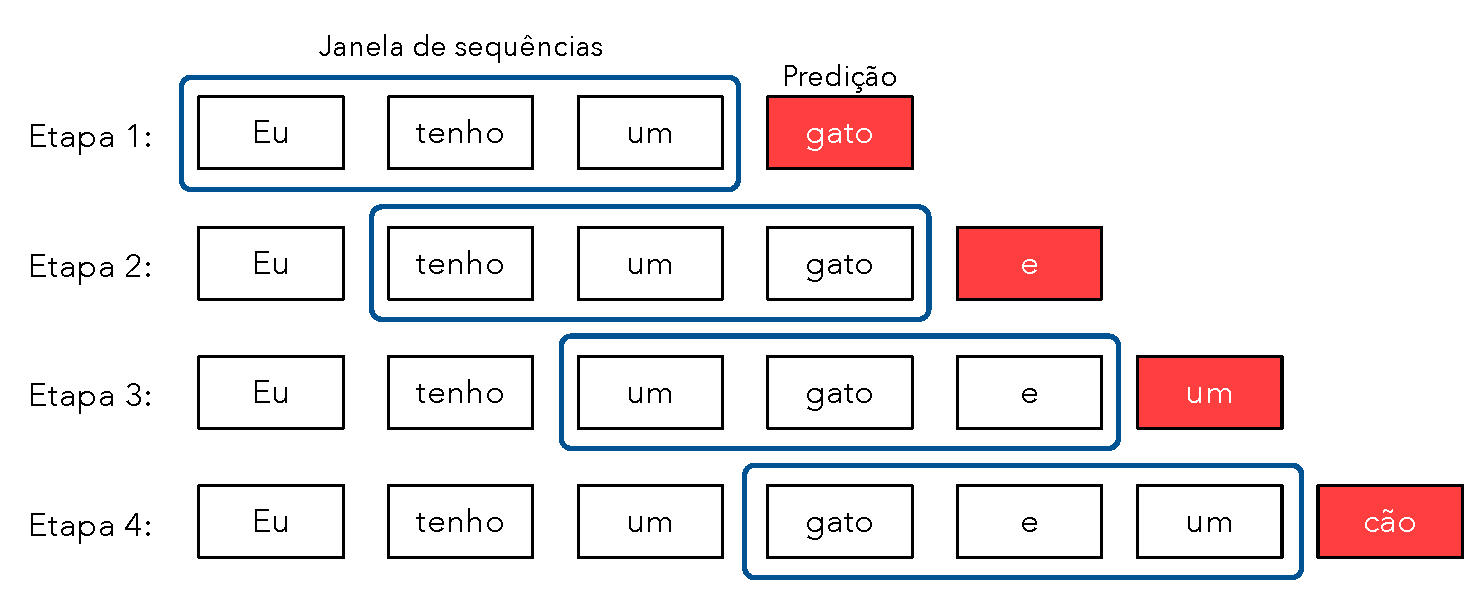
\includegraphics[scale=0.425]{figs/text_generation.eps}	
		\label{f.causal_lm}
		\caption{Processo de modelagem de linguagem causal.}
	\end{figure}
	Código: \url{https://github.com/gugarosa/text_augmenter/tree/master/applications/causal}
\end{frame}

\begin{frame}{\emph{Bot} para Augmentação de Dados}
	\begin{figure}[!ht]
		\centering
		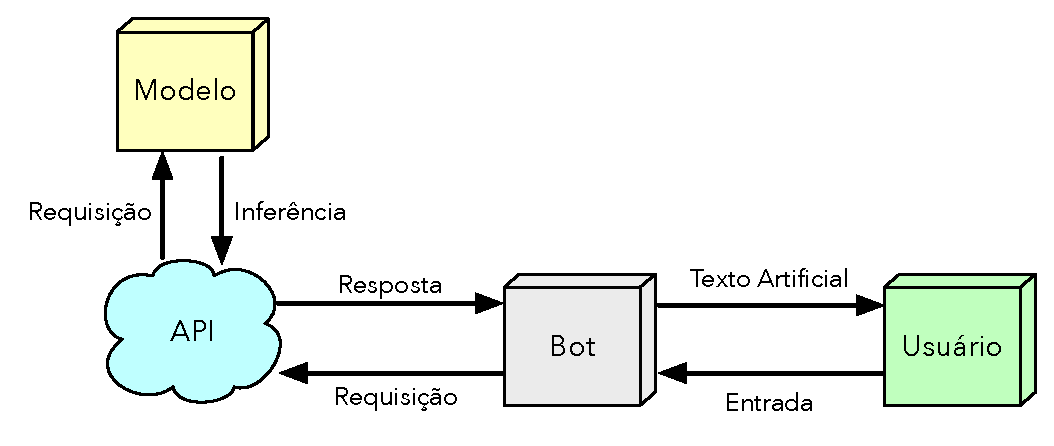
\includegraphics[scale=0.45]{figs/bot.eps}	
		\label{f.bot}
		\caption{Fluxograma de um \emph{bot} para augmentação de dados.}
	\end{figure}
	Código: \url{https://github.com/gugarosa/text_augmenter/tree/master/applications/bot}
	\\~\\
	Telegram: @RecognaBot
\end{frame}

\section{Conclusão}
\label{s.conclusion}

\begin{frame}{Conclusão}
	Lorem ipsum ...
\end{frame}

% Defines the references and its slides
\section*{Referências}
\begin{frame}[allowframebreaks]
	\bibliography{references}
	\bibliographystyle{abbrv}
\end{frame}

% Defines the standout finishing slide
\begin{frame}[plain,standout]
	Perguntas?
	\\~\\
	Obrigado pela atenção!
\end{frame}

% Ends the document
\end{document}